\documentclass{article}

\usepackage[margin=2.5cm]{geometry}

\usepackage{amsmath}
\usepackage{graphicx}
\usepackage{tabularx}

\usepackage{booktabs}
\usepackage[flushleft]{threeparttable}

\usepackage{caption} 
\captionsetup[table]{skip=10pt}  % more space between the caption and table

\usepackage{dcolumn}
% First argument - the separator used to align the numbers, the second - how this separator appears in the output,
% the last argument corresponds to a maximum number of decimal places in the column 2.3 means the column is centered around a number like xx.yyy
\newcolumntype{d}[1]{D{.}{.}{#1}}
\newcolumntype{t}{D{.}{.}{2}}

% Shortcut to a single-entry multicolumn to comply with `dcolumn` rules -- i.e. to be able to enter strings into dcolumns
\newcommand\mc[1]{\multicolumn{1}{c}{$\text{#1}$}}


\begin{document}


% simple unaligned version
\begin{table}[ht!]
\setlength\tabcolsep{6pt}
\footnotesize
  \centering
  \caption{\normalsize Descriptive Statistics: Monthly Returns Jan 2019 -- Jul 2020}

	\begin{tabular}{lccccccc}

	\toprule
			&  & \multicolumn{2}{c}{$\text{Tech}$} & \multicolumn{2}{c}{$\text{Banks}$} & \multicolumn{2}{c}{$\text{Auto}$} \\[0.25ex]

	\cmidrule(l{10pt}r{10pt}){3-4} \cmidrule(l{10pt}r{10pt}){5-6} \cmidrule(l{10pt}r{10pt}){7-8}

	Asset &\mc{SPY} &\mc{AAPL} &\mc{MSFT} &\mc{JPM} & \mc{GS} & \mc{TSLA} &\mc{GM} \\[0.25ex]

	\midrule
	\multicolumn{8}{l}{Panel A: Descriptive statistics} \\[0.25ex]
	\midrule 
									
	Mean		&1.73	&5.80	&4.00	&0.63	&1.60	&10.13	&-0.60 \\[0.25ex]
	Median		&2.21	&7.64	&3.12	&3.74	&2.97	&6.76	&-0.85 \\[0.25ex]
	Std. dev.	&5.78	&8.40	&5.14	&8.71	&10.40	&22.62	&11.44 \\[0.25ex]
	Skewness	&-0.81	&-1.06	&0.01	&-1.02	&-0.58	&0.44	&-0.68 \\[0.25ex]
	Kurtosis	&1.36	&0.51	&-0.46	&1.55	&0.79	&-0.55	&1.73 \\[0.25ex]

	 												
	\midrule
	\multicolumn{8}{l}{Panel B: Correlation matrix}\\[0.25ex]
	\midrule


	$\text{SPY}$	&1.0  	&0.83	&0.71	&0.85	&0.94	&0.50	&0.85	\\[0.25ex]
	$\text{AAPL}$	&0.83	&1.0  	&0.71	&0.68	&0.73	&0.64	&0.61 	\\[0.25ex]
	$\text{MSFT}$	&0.71	&0.71	&1.0  	&0.56	&0.67	&0.51	&0.47 	\\[0.25ex]
	$\text{JPM}$	&0.85	&0.68	&0.56	&1.0  	&0.84	&0.30	&0.8	\\[0.25ex]
	$\text{GS}$ 	&0.94	&0.73	&0.67	&0.84	&1.0  	&0.46	&0.89	\\[0.25ex]
	$\text{TSLA}$	&0.50	&0.64	&0.51	&0.30	&0.46	&1.0  	&0.28	\\[0.25ex]
	$\text{GM}$	    &0.85	&0.61	&0.47	&0.80	&0.89	&0.28	&1.0 	\\[0.25ex]

	\bottomrule

    \end{tabular}

\end{table}


% dcolumn version: aligned by '.' + less space between columns from the same sector
\begin{table}[ht!]
\setlength\tabcolsep{3pt}
\footnotesize
  \centering
  \caption{\normalsize Descriptive Statistics: Monthly Returns Jan 2019 -- Jul 2020}

	\begin{tabular}{l@{\hskip 15pt}d{1}@{\hskip 15pt}d{2}d{2}@{\hskip 15pt}d{2}d{2}@{\hskip 15pt}d{2}d{2}}

	\toprule
			&  & \multicolumn{2}{c}{$\text{Tech}$} & \multicolumn{2}{c}{$\text{Banks}$} & \multicolumn{2}{c}{$\text{Auto}$} \\[0.25ex]

	\cmidrule(l{10pt}r{10pt}){3-4} \cmidrule(l{10pt}r{10pt}){5-6} \cmidrule(l{10pt}r{10pt}){7-8}

	Asset &\mc{SPY} &\mc{AAPL} &\mc{MSFT} &\mc{JPM} & \mc{GS} & \mc{TSLA} &\mc{GM} \\[0.25ex]

	\midrule
	\multicolumn{8}{l}{Panel A: Descriptive statistics} \\[0.25ex]
	\midrule 
									
	Mean		&1.73	&5.80	&4.00	&0.63	&1.60	&10.13	&-0.60 \\[0.25ex]
	Median		&2.21	&7.64	&3.12	&3.74	&2.97	&6.76	&-0.85 \\[0.25ex]
	Std. dev.	&5.78	&8.40	&5.14	&8.71	&10.40	&22.62	&11.44 \\[0.25ex]
	Skewness	&-0.81	&-1.06	&0.01	&-1.02	&-0.58	&0.44	&-0.68 \\[0.25ex]
	Kurtosis	&1.36	&0.51	&-0.46	&1.55	&0.79	&-0.55	&1.73 \\[0.25ex]

	 												
	\midrule
	\multicolumn{8}{l}{Panel B: Correlation matrix}\\[0.25ex]
	\midrule


	SPY		&	  	&		&		&		&		&		&	 \\[0.25ex]
	AAPL	&0.83	&	  	&		&		&		&		&	 \\[0.25ex]
	MSFT	&0.71	&0.71	&	  	&		&		&		& 	 \\[0.25ex]
	JPM		&0.85	&0.68	&0.56	&	  	&		&		&	 \\[0.25ex]
	GS 		&0.94	&0.73	&0.67	&0.84	&	  	&		&	 \\[0.25ex]
	TSLA	&0.50	&0.64	&0.51	&0.30	&0.46	&	  	&	 \\[0.25ex]
	GM	    &0.85	&0.61	&0.47	&0.80	&0.89	&0.28	&  	 \\[0.25ex]

	\bottomrule

    \end{tabular}

\end{table}

% ---------------------------------------------------------------------------
\pagebreak
\begin{table}[h!]
	\setlength\tabcolsep{3pt}
	\small
	\centering
	\caption{\normalsize Betas: table form}
	\begin{tabularx}{0.8\textwidth}{Xtttttttttt}
\toprule
{} & \multicolumn{1}{c}{AAPL} & \multicolumn{1}{c}{CVX} & \multicolumn{1}{c}{DAL} & \multicolumn{1}{c}{GM} & \multicolumn{1}{c}{GS} & \multicolumn{1}{c}{JPM} & \multicolumn{1}{c}{LUV} & \multicolumn{1}{c}{MSFT} & \multicolumn{1}{c}{TSLA} & \multicolumn{1}{c}{XOM} \\
\midrule
daily    &                     1.06 &                    1.16 &                    1.27 &                   1.25 &                   1.34 &                    1.32 &                    1.07 &                     1.11 &                     1.27 &                    1.00 \\
         &                   (0.02) &                  (0.02) &                  (0.04) &                 (0.03) &                 (0.02) &                  (0.02) &                  (0.03) &                   (0.02) &                   (0.06) &                  (0.02) \\
monthly  &                     1.09 &                    1.20 &                    1.16 &                   1.55 &                   1.62 &                    1.50 &                    1.10 &                     0.86 &                     1.01 &                    1.19 \\
         &                   (0.16) &                  (0.11) &                  (0.22) &                 (0.16) &                 (0.14) &                  (0.12) &                  (0.19) &                   (0.12) &                   (0.38) &                  (0.10) \\
annually &                     0.87 &                    1.33 &                   -0.38 &                   1.77 &                   1.22 &                    1.35 &                    0.26 &                     1.13 &                    -0.30 &                    0.74 \\
         &                   (0.57) &                  (0.44) &                  (1.22) &                 (0.52) &                 (0.61) &                  (0.43) &                  (1.01) &                   (0.34) &                   (2.18) &                  (0.50) \\
\bottomrule
\end{tabularx}

\end{table}

\vspace{24pt}

\begin{figure}[h!]
	\caption{Betas: heatmap form}
	\centering
	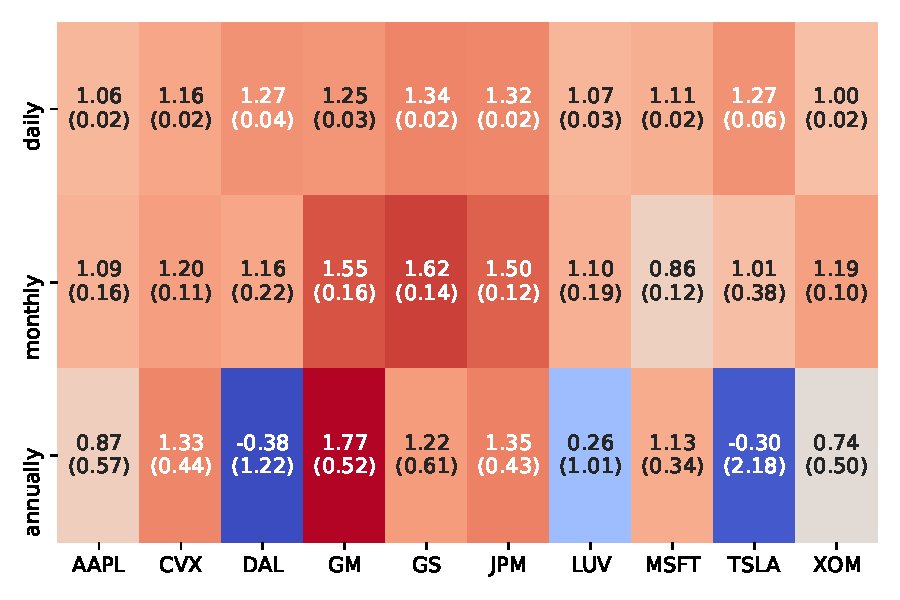
\includegraphics{betas-hmap.pdf}
\end{figure}


\end{document}